\documentclass[border=12pt]{standalone}
\usepackage{tikz}
\usetikzlibrary{shapes.geometric, arrows.meta, positioning, calc, fit, backgrounds}
\usepackage{fontspec}
\usepackage{amsmath,amssymb}
\setmainfont{DejaVu Sans}

\begin{document}
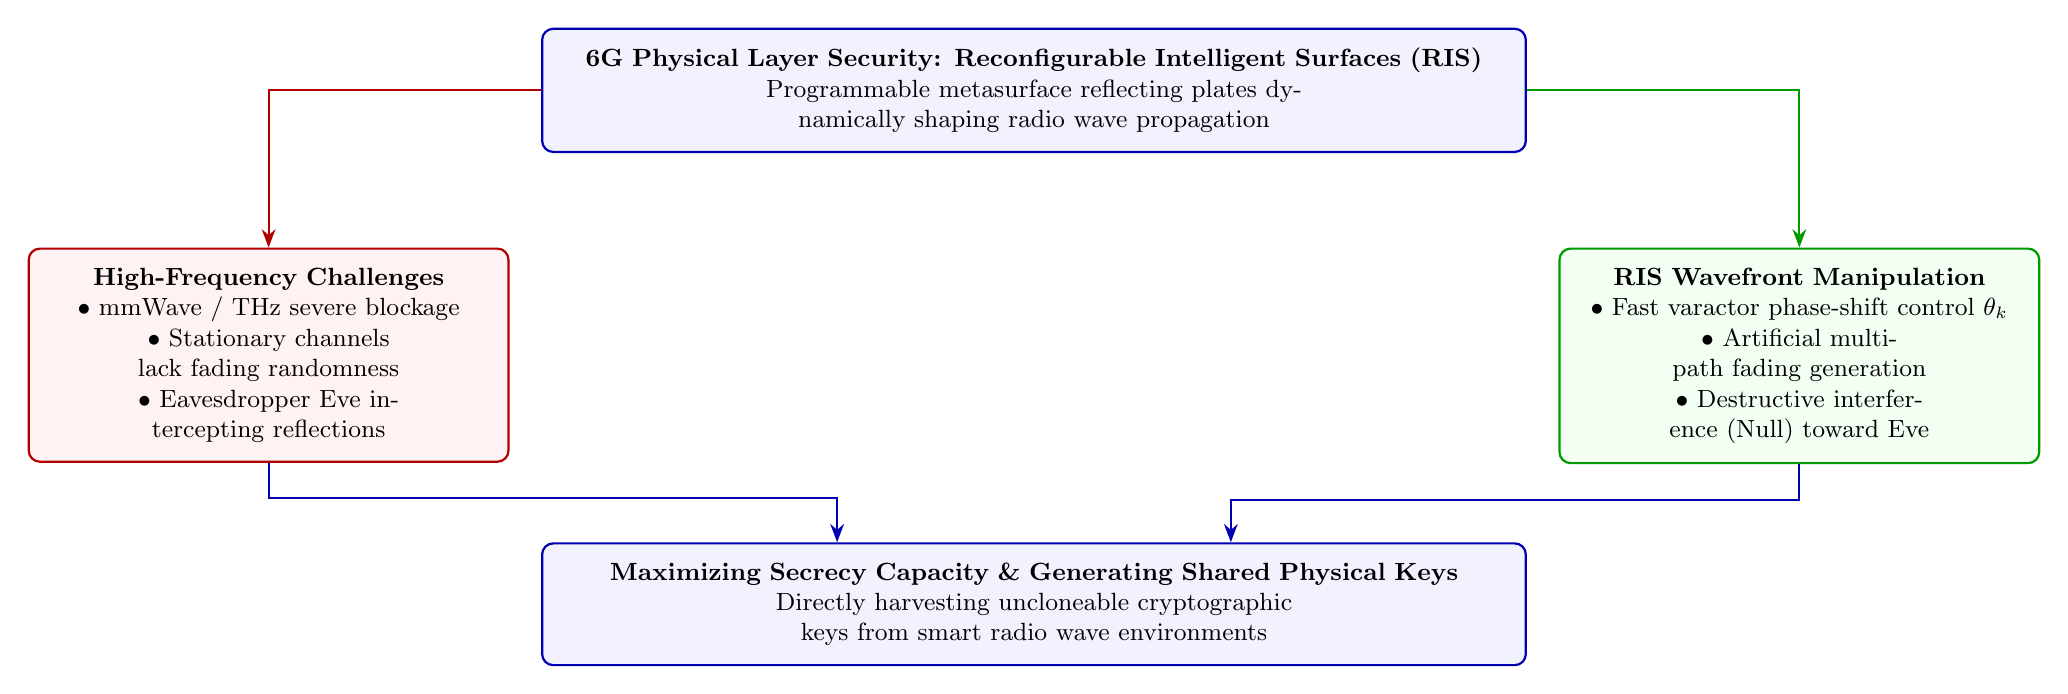
\begin{tikzpicture}[
    font=\small,
    >=Stealth,
    node distance=1.2cm,
    block/.style={rectangle, draw=blue!70!black, fill=blue!5, rounded corners=4pt, thick, align=center, inner sep=7pt},
    alertblock/.style={rectangle, draw=red!70!black, fill=red!5, rounded corners=4pt, thick, align=center, inner sep=7pt},
    greenblock/.style={rectangle, draw=green!60!black, fill=green!5, rounded corners=4pt, thick, align=center, inner sep=7pt},
    amberblock/.style={rectangle, draw=orange!80!black, fill=orange!5, rounded corners=4pt, thick, align=center, inner sep=7pt}
]

\node[block, text width=12cm] (top) {\textbf{6G Physical Layer Security: Reconfigurable Intelligent Surfaces (RIS)}\\Programmable metasurface reflecting plates dynamically shaping radio wave propagation};

\node[alertblock, below left=1.2cm and 0.4cm of top, text width=5.6cm] (threat) {\textbf{High-Frequency Challenges}\\$\bullet$ mmWave / THz severe blockage\\$\bullet$ Stationary channels lack fading randomness\\$\bullet$ Eavesdropper Eve intercepting reflections};

\node[greenblock, below right=1.2cm and 0.4cm of top, text width=5.6cm] (ris_sol) {\textbf{RIS Wavefront Manipulation}\\$\bullet$ Fast varactor phase-shift control $\theta_k$\\$\bullet$ Artificial multipath fading generation\\$\bullet$ Destructive interference (Null) toward Eve};

\node[block, below=1.0cm of $(threat.south)!0.5!(ris_sol.south)$, text width=12cm] (bottom) {\textbf{Maximizing Secrecy Capacity \& Generating Shared Physical Keys}\\Directly harvesting uncloneable cryptographic keys from smart radio wave environments};

\draw[->, thick, red!70!black] (top) -| (threat);
\draw[->, thick, green!60!black] (top) -| (ris_sol);
\draw[->, thick, blue!70!black] (threat.south) -- ++(0,-0.45) -| ([xshift=-2.5cm]bottom.north);
\draw[->, thick, blue!70!black] (ris_sol.south) -- ++(0,-0.45) -| ([xshift=2.5cm]bottom.north);

\end{tikzpicture}
\end{document}
